%% (Master) Thesis template
% Template version used: v1.4
%
% Largely adapted from Adrian Nievergelt's template for the ADPS
% (lecture notes) project.


%% We use the memoir class because it offers a many easy to use features.
\documentclass[11pt,a4paper,titlepage,oneside]{memoir}

%% Packages
%% ========

%% LaTeX Font encoding -- DO NOT CHANGE
\usepackage[OT1]{fontenc}

%% Babel provides support for languages.  'english' uses British
%% English hyphenation and text snippets like "Figure" and
%% "Theorem". Use the option 'ngerman' if your document is in German.
%% Use 'american' for American English.  Note that if you change this,
%% the next LaTeX run may show spurious errors.  Simply run it again.
%% If they persist, remove the .aux file and try again.
\usepackage[english]{babel}

%% Input encoding 'utf8'. In some cases you might need 'utf8x' for
%% extra symbols. Not all editors, especially on Windows, are UTF-8
%% capable, so you may want to use 'latin1' instead.
\usepackage[utf8]{inputenc}

%% This changes default fonts for both text and math mode to use Herman Zapfs
%% excellent Palatino font.  Do not change this.
\usepackage[sc]{mathpazo}

%% The AMS-LaTeX extensions for mathematical typesetting.  Do not
%% remove.
\usepackage{amsmath,amssymb,amsfonts,mathrsfs}

%% NTheorem is a reimplementation of the AMS Theorem package. This
%% will allow us to typeset theorems like examples, proofs and
%% similar.  Do not remove.
%% NOTE: Must be loaded AFTER amsmath, or the \qed placement will
%% break
\usepackage[amsmath,thmmarks]{ntheorem}

%% LaTeX' own graphics handling
\usepackage{graphicx}

%% We unfortunately need this for the Rules chapter.  Remove it
%% afterwards; or at least NEVER use its underlining features.
\usepackage{soul}

%% This allows you to add .pdf files. It is used to add the
%% declaration of originality.
\usepackage{pdfpages}

%% Some more packages that you may want to use.  Have a look at the
%% file, and consult the package docs for each.
%% See the TeXed file for more explanations

%% [OPT] Multi-rowed cells in tabulars
%\usepackage{multirow}

%% [REC] Intelligent cross reference package. This allows for nice
%% combined references that include the reference and a hint to where
%% to look for it.
\usepackage{varioref}

%% [OPT] Easily changeable quotes with \enquote{Text}
%\usepackage[german=swiss]{csquotes}

%% [REC] Format dates and time depending on locale
\usepackage{datetime}

%% [OPT] Provides a \cancel{} command to stroke through mathematics.
%\usepackage{cancel}

%% [NEED] This allows for additional typesetting tools in mathmode.
%% See its excellent documentation.
\usepackage{mathtools}

%% [ADV] Conditional commands
%\usepackage{ifthen}

%% [OPT] Manual large braces or other delimiters.
%\usepackage{bigdelim, bigstrut}

%% [REC] Alternate vector arrows. Use the command \vv{} to get scaled
%% vector arrows.
\usepackage[h]{esvect}

%% [NEED] Some extensions to tabulars and array environments.
\usepackage{array}

%% [OPT] Postscript support via pstricks graphics package. Very
%% diverse applications.
%\usepackage{pstricks,pst-all}

%% [?] This seems to allow us to define some additional counters.
%\usepackage{etex}

%% [ADV] XY-Pic to typeset some matrix-style graphics
%\usepackage[all]{xy}

%% [OPT] This is needed to generate an index at the end of the
%% document.
%\usepackage{makeidx}

%% [OPT] Fancy package for source code listings.  The template text
%% needs it for some LaTeX snippets; remove/adapt the \lstset when you
%% remove the template content.
\usepackage{listings}
\lstset{language=TeX,basicstyle={\normalfont\ttfamily}}

%% [REC] Fancy character protrusion.  Must be loaded after all fonts.
\usepackage[activate]{pdfcprot}

%% [REC] Nicer tables.  Read the excellent documentation.
\usepackage{booktabs}


%% Our layout configuration.  DO NOT CHANGE.
%% Memoir layout setup

%% NOTE: You are strongly advised not to change any of them unless you
%% know what you are doing.  These settings strongly interact in the
%% final look of the document.

% Dependencies
\usepackage{utils/ETHlogo}

% Turn extra space before chapter headings off.
\setlength{\beforechapskip}{0pt}

\nonzeroparskip
\parindent=0pt
\defaultlists

% Chapter style redefinition
\makeatletter

\if@twoside
  \pagestyle{Ruled}
  \copypagestyle{chapter}{Ruled}
\else
  \pagestyle{ruled}
  \copypagestyle{chapter}{ruled}
\fi
\makeoddhead{chapter}{}{}{}
\makeevenhead{chapter}{}{}{}
\makeheadrule{chapter}{\textwidth}{0pt}
\copypagestyle{abstract}{empty}

\makechapterstyle{bianchimod}{%
  \chapterstyle{default}
  \renewcommand*{\chapnamefont}{\normalfont\Large\sffamily}
  \renewcommand*{\chapnumfont}{\normalfont\Large\sffamily}
  \renewcommand*{\printchaptername}{%
    \chapnamefont\centering\@chapapp}
  \renewcommand*{\printchapternum}{\chapnumfont {\thechapter}}
  \renewcommand*{\chaptitlefont}{\normalfont\huge\sffamily}
  \renewcommand*{\printchaptertitle}[1]{%
    \hrule\vskip\onelineskip \centering \chaptitlefont\textbf{\vphantom{gyM}##1}\par}
  \renewcommand*{\afterchaptertitle}{\vskip\onelineskip \hrule\vskip
    \afterchapskip}
  \renewcommand*{\printchapternonum}{%
    \vphantom{\chapnumfont {9}}\afterchapternum}}

% Use the newly defined style
\chapterstyle{bianchimod}

\setsecheadstyle{\Large\bfseries\sffamily}
\setsubsecheadstyle{\large\bfseries\sffamily}
\setsubsubsecheadstyle{\bfseries\sffamily}
\setparaheadstyle{\normalsize\bfseries\sffamily}
\setsubparaheadstyle{\normalsize\itshape\sffamily}
\setsubparaindent{0pt}

% Set captions to a more separated style for clearness
\captionnamefont{\sffamily\bfseries\footnotesize}
\captiontitlefont{\sffamily\footnotesize}
\setlength{\intextsep}{16pt}
\setlength{\belowcaptionskip}{1pt}

% Set section and TOC numbering depth to subsection
\setsecnumdepth{subsection}
\settocdepth{subsection}

%% Titlepage adjustments
\pretitle{\vspace{0pt plus 0.7fill}\begin{center}\HUGE\sffamily\bfseries}
\posttitle{\end{center}\par}
\preauthor{\par\begin{center}\let\and\\\Large\sffamily}
\postauthor{\end{center}}
\predate{\par\begin{center}\Large\sffamily}
\postdate{\end{center}}

\def\@advisors{}
\newcommand{\advisors}[1]{\def\@advisors{#1}}
\def\@department{}
\newcommand{\department}[1]{\def\@department{#1}}
\def\@thesistype{}
\newcommand{\thesistype}[1]{\def\@thesistype{#1}}

\renewcommand{\maketitlehooka}{\noindent\ETHlogo[2in]}

\renewcommand{\maketitlehookb}{\vspace{1in}%
  \par\begin{center}\Large\sffamily\@thesistype\end{center}}

\renewcommand{\maketitlehookd}{%
  \vfill\par
  \begin{flushright}
    \sffamily
    \@advisors\par
    \@department, ETH Z\"urich
  \end{flushright}
}

\checkandfixthelayout

\setlength{\droptitle}{-48pt}

\makeatother

% This defines how theorems should look. Best leave as is.
\theoremstyle{plain}
\setlength\theorempostskipamount{0pt}

%%% Local Variables:
%%% mode: latex
%%% TeX-master: "thesis"
%%% End:


%% Theorem environments.  You will have to adapt this for a German
%% thesis.
%% Theorem-like environments

%% This can be changed according to language. You can comment out the ones you
%% don't need.

\numberwithin{equation}{chapter}

%% German theorems
%\newtheorem{satz}{Satz}[chapter]
%\newtheorem{beispiel}[satz]{Beispiel}
%\newtheorem{bemerkung}[satz]{Bemerkung}
%\newtheorem{korrolar}[satz]{Korrolar}
%\newtheorem{definition}[satz]{Definition}
%\newtheorem{lemma}[satz]{Lemma}
%\newtheorem{proposition}[satz]{Proposition}

%% English variants
\newtheorem{theorem}{Theorem}[chapter]
\newtheorem{example}[theorem]{Example}
\newtheorem{remark}[theorem]{Remark}
\newtheorem{corollary}[theorem]{Corollary}
\newtheorem{definition}[theorem]{Definition}
\newtheorem{lemma}[theorem]{Lemma}
\newtheorem{proposition}[theorem]{Proposition}

%% Proof environment with a small square as a "qed" symbol
\theoremstyle{nonumberplain}
\theorembodyfont{\normalfont}
\theoremsymbol{\ensuremath{\square}}
\newtheorem{proof}{Proof}
%\newtheorem{beweis}{Beweis}


%% Helpful macros.
%% Custom commands
%% ===============

%% Special characters for number sets, e.g. real or complex numbers.
\newcommand{\C}{\mathbb{C}}
\newcommand{\K}{\mathbb{K}}
\newcommand{\N}{\mathbb{N}}
\newcommand{\Q}{\mathbb{Q}}
\newcommand{\R}{\mathbb{R}}
\newcommand{\Z}{\mathbb{Z}}
\newcommand{\X}{\mathbb{X}}

%% Fixed/scaling delimiter examples (see mathtools documentation)
\DeclarePairedDelimiter\abs{\lvert}{\rvert}
\DeclarePairedDelimiter\norm{\lVert}{\rVert}

%% Use the alternative epsilon per default and define the old one as \oldepsilon
\let\oldepsilon\epsilon
\renewcommand{\epsilon}{\ensuremath\varepsilon}

%% Also set the alternate phi as default.
\let\oldphi\phi
\renewcommand{\phi}{\ensuremath{\varphi}}


%% Make document internal hyperlinks wherever possible. (TOC, references)
%% This MUST be loaded after varioref, which is loaded in 'extrapackages'
%% above.  We just load it last to be safe.
\usepackage[linkcolor=black,colorlinks=true,citecolor=black,filecolor=black]{hyperref}

%% Support Mathematica cells
\usepackage{mmacells}

%% Keep floats within sections
\let\origsection\section
\usepackage[section]{placeins}

%% Command for an imaginary i
\newcommand{\iu}{{i\mkern1mu}}

%% Command for a ditto symbol
\usepackage{tikz}
\newcommand{\dittotikz}{%
    \tikz{
        \draw [line width=0.12ex] (-0.2ex,0) -- +(0,0.8ex)
            (0.2ex,0) -- +(0,0.8ex);
        \draw [line width=0.08ex] (-0.6ex,0.4ex) -- +(-1.5em,0)
            (0.6ex,0.4ex) -- +(1.5em,0);
    }%
}

%% Defining checkmark and crossmark
\usepackage{pifont}% http://ctan.org/pkg/pifont
\newcommand{\cmark}{\ding{51}}%
\newcommand{\xmark}{\ding{55}}%

%% Document information
%% ====================

\title{Supervisory Control and Data Acquisition system of the n2EDM experiment}
\author{Konstantin Nesterov}
\thesistype{Master's Thesis}
\advisors{Advisors: Prof.\ Dr.\ K. S. Kirch, Dr.\ Jochen Krempel}
\department{Department of Physics}
\date{\today}

\begin{document}

\frontmatter

%% Title page is autogenerated from document information above.  DO
%% NOT CHANGE.
\begin{titlingpage}
  \calccentering{\unitlength}
  \begin{adjustwidth*}{\unitlength-24pt}{-\unitlength-24pt}
    \maketitle
  \end{adjustwidth*}
\end{titlingpage}

%% The abstract of your thesis.  Edit the file as needed.
%\begin{abstract}
  Just as nowadays no serious experiment can be built and conducted by a single person, the experiment itself cannot consist of a single tool. The n2EDM experiment aims to achieve an ambitious goal: to measure the electric dipole moment of a neutron with a new level of precision. Such challenging project demands the need for the complex and well-connected system. This thesis intends to describe the development of new and improvement of existing components, such as:
  \begin{itemize}
  	\item \textbf{COM handler} --- an adapter translating the POSIX pipes to the TCP/IP connections. Almost every node in the DAQ system is connected with others through it.
  	\item \textbf{Sequencer} --- a software node orchestrating other nodes. It follows the user-generated script allowing one to describe the reproducible behaviour of the whole DAQ system with a human-readable set of commands.
  	\item \textbf{Proxy for the remote magnetometers} --- a smart bridge between the pool of the remote magnetometers and a standard TCP/IP interface of the COM handler.
  	\item \textbf{Surrounding field compensation system} --- a system for the active stabilisation of the magnetic field. It uses the a set of controlled coils to minimise the magnetic fluctuations in the area of the n2EDM experiment.
  \end{itemize}
  These pieces are essential for the n2EDM experiment to function, so the aim was to make them error-resistant, extendable and easy to support for the future developers.
  
  \vfill
  
  Check the source at\enskip\url{https://github.com/wasd171/diploma-msc}

\end{abstract}


%% TOC with the proper setup, do not change.
\cleartorecto
\tableofcontents
\mainmatter

%% Your real content!
%\chapter{Introduction}
\label{chapter:introduction}

\setlength{\epigraphwidth}{0.43\textwidth}
\epigraph{
Out of S. Okubo's effect\\
At high temperature\\
A fur coat is sewed for the Universe\\
Shaped for its crooked figure
}{A. D. Sakharov \cite{Sakharov1991}}

We interact with matter every day. Even you, the reader, are probably made out of matter! However, antimatter is so rare that it is considered to cost a few hundred millions Swiss francs per gram \cite{DeRujula2001}, making it the most expensive substance in the universe. Why does such a stunning difference in the abundance exist?

First step to solving this problem is to define what are the required conditions that would allow the disbalance to evolve. Those conditions \cite{Dubbers2011} were described \cite{Sakharov1991} by Andrei Sakharov in 1967:

\begin{itemize}
	\item Violation of baryon number conservation
	\item \textit{C}- and \textit{CP}-symmetry violation
	\item Processes take place far from thermal equilibrium
\end{itemize}

Let's take a look at the \textit{CP}-symmetry and prove that a non-zero electric dipole moment of an elementary particle would indeed break it. We would select neutron as a particle of choice.

The neutron in the ground state has spin of $I = 1/2$ and can be characterised completely by a single quantum number of a spin projection $m_I = \pm 1/2$. We can write down a Hamiltonian \cite{Golub1994} of this neutron in external electric and magnetic fields $\vec{E}$ and $\vec{B}$:

\begin{equation}
	\mathcal{H} = -\frac{d_n \vec{I} \cdot \vec{E} + \mu_n \vec{I} \cdot \vec{B}}{I}
	\label{eq:neutron_hamiltonian}
\end{equation}

with $d_n$ and $\mu_n$ being the electric and magnetic moments of the neutron \cite{Golub1972}.

It does not make sense to discuss the potential violation of the symmetries before we define them.  Fundamental symmetries are blended into the fabric of our Universe by providing sufficient conditions \cite{Noether1918} for the conservation laws. In our analysis we would consider three symmetries of the Standard Model: \textit{C}, \textit{P} and \textit{T}.

\begin{itemize}
	\item (C)harge –-- replaces every particle with its antiparticle: $q \rightarrow -q$
	\item (P)arity --- inverts the physical space: $\vec{r} \rightarrow -\vec{r}$
	\item (T)ime --- turns the time back: $t \rightarrow -t$
\end{itemize}

How would the \textit{P} and \textit{T} inversions affect \cite{Dubbers2011} the Hamiltonian from Eq. \ref{eq:neutron_hamiltonian}?

Parity transformation only act on a polar vector of the electric field: $\vec{E} \rightarrow -\vec{E}$, both $\vec{B}$ and $\vec{I}$ are conserved. This brings us to
\begin{equation}
	\textit{P}\mathcal{H} = -\frac{d_n \vec{I} \cdot \left(-\vec{E}\right) + \mu_n \vec{I} \cdot \vec{B}}{I} \neq \mathcal{H}
	\label{eq:neutron_hamiltonian_P}
\end{equation}

Time reversal would affect only axial vectors $\vec{B}$ and $\vec{I}$: $\vec{B} \rightarrow -\vec{B},\ \vec{I} \rightarrow -\vec{I}$, the field $\vec{E}$ is left as is:
\begin{equation}
	\textit{T}\mathcal{H} = -\frac{d_n \left(-\vec{I}\right) \cdot \vec{E} + \mu_n \left(-\vec{I}\right) \cdot \left( -\vec{B} \right)}{I} \neq \mathcal{H}
	\label{eq:neutron_hamiltonian_T}
\end{equation}

Assuming that the \textit{CPT} invariance \cite{Schwinger1951} is conserved, we derive the violation of a \textit{CP}-symmetry, which provides us motivation to measure the EDM of the neutron.

\textit{"Wait a minute,"} could have said an attentive reader at this point. "Does not Standard Model predict a non-zero EDM of the neutron already? I am still not convinced why would you want to conduct this experiment."

And an attentive reader would have had a completely fair point! Indeed, Standard Model predicts \cite{Khriplovich1982} the following:
\begin{equation}
	d_n \approx 2 \cdot 10^{-32}\ e \cdot \text{cm}
\end{equation}

However, we would still like to measure $d_n$ for the reasons listed below:
\begin{itemize}
	\item The only way to prove the theory is to check it experimentally. So far no one has measured $d_n$ with a precision close to the predicted value
	\item The result that can be achieved by using Standard Model is too weak to explain the baryogenesis \cite{Dubbers2011}, yet baryogenesis has clearly happened
	\item If we go beyond Standard Model to find a mechanism, through which the Universe as we know it could have been formed, we need to cut off theories that do not agree with experimental data. This is something that this experiment does perfectly: on the Fig. \ref{fig:edm_history} one can see all theoretical models that the measurement of the neutron EDM has ruled out, allowing the scientists to focus on more prominent theories.
\end{itemize}

\begin{figure}[h]
	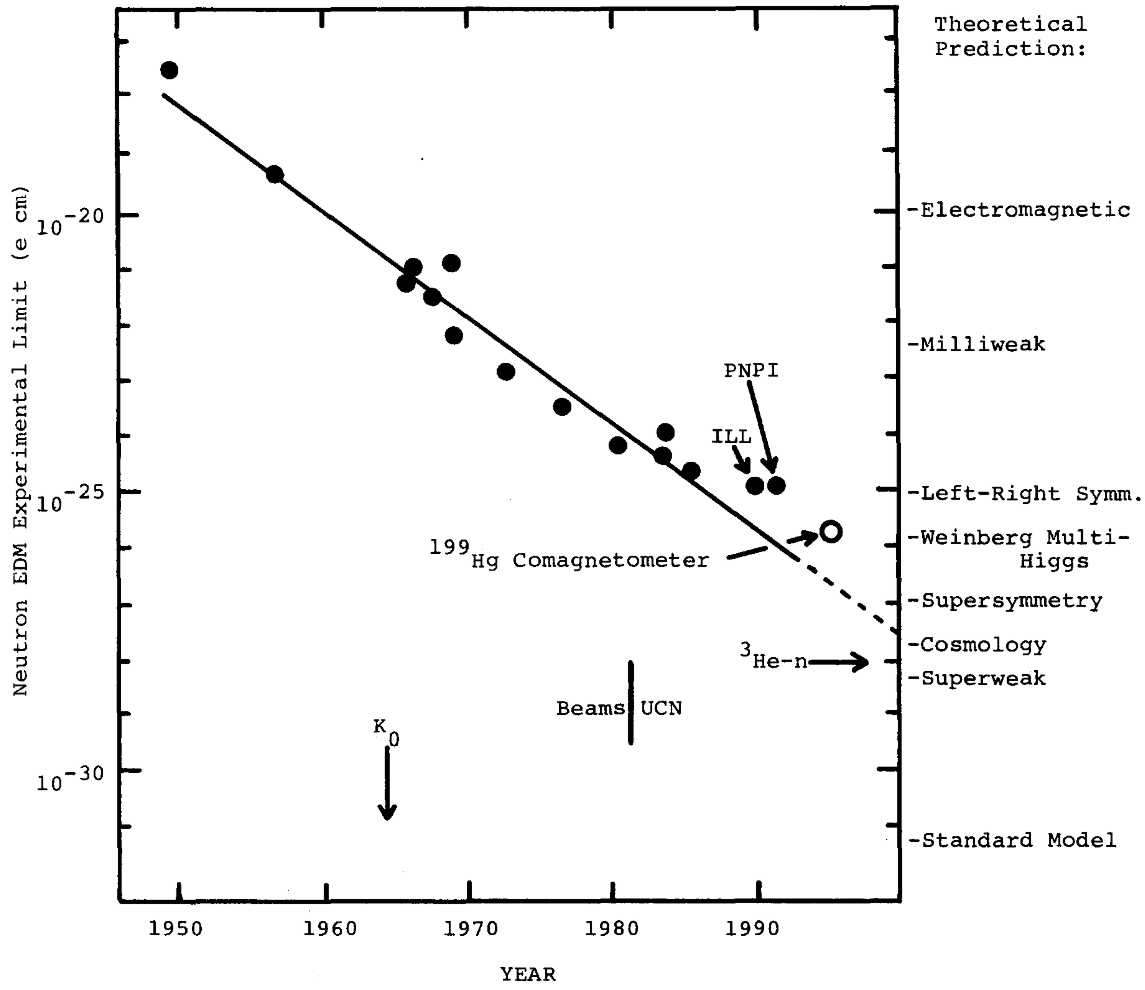
\includegraphics[width=\textwidth]{img/history_of_nedm_measurements}
	\caption{Measurement history of the neutron EDM \cite{Golub1994}}
	\label{fig:edm_history}
\end{figure}

Hopefully these reasons would convince even the most demanding reader in the need to conduct the n2EDM experiment. But what is \textit{n2EDM} exactly? We will try to explain that in the next chapter.

%\input{theory}
%\input{design}
%\input{validation}
%\input{results}
%\input{outlook}
%\input{conclusion}
%\input{additions}

\appendix
%\input{appendix_macalpine}
%\input{appendix_siverns}

\backmatter

\bibliographystyle{plain}
\bibliography{refs}

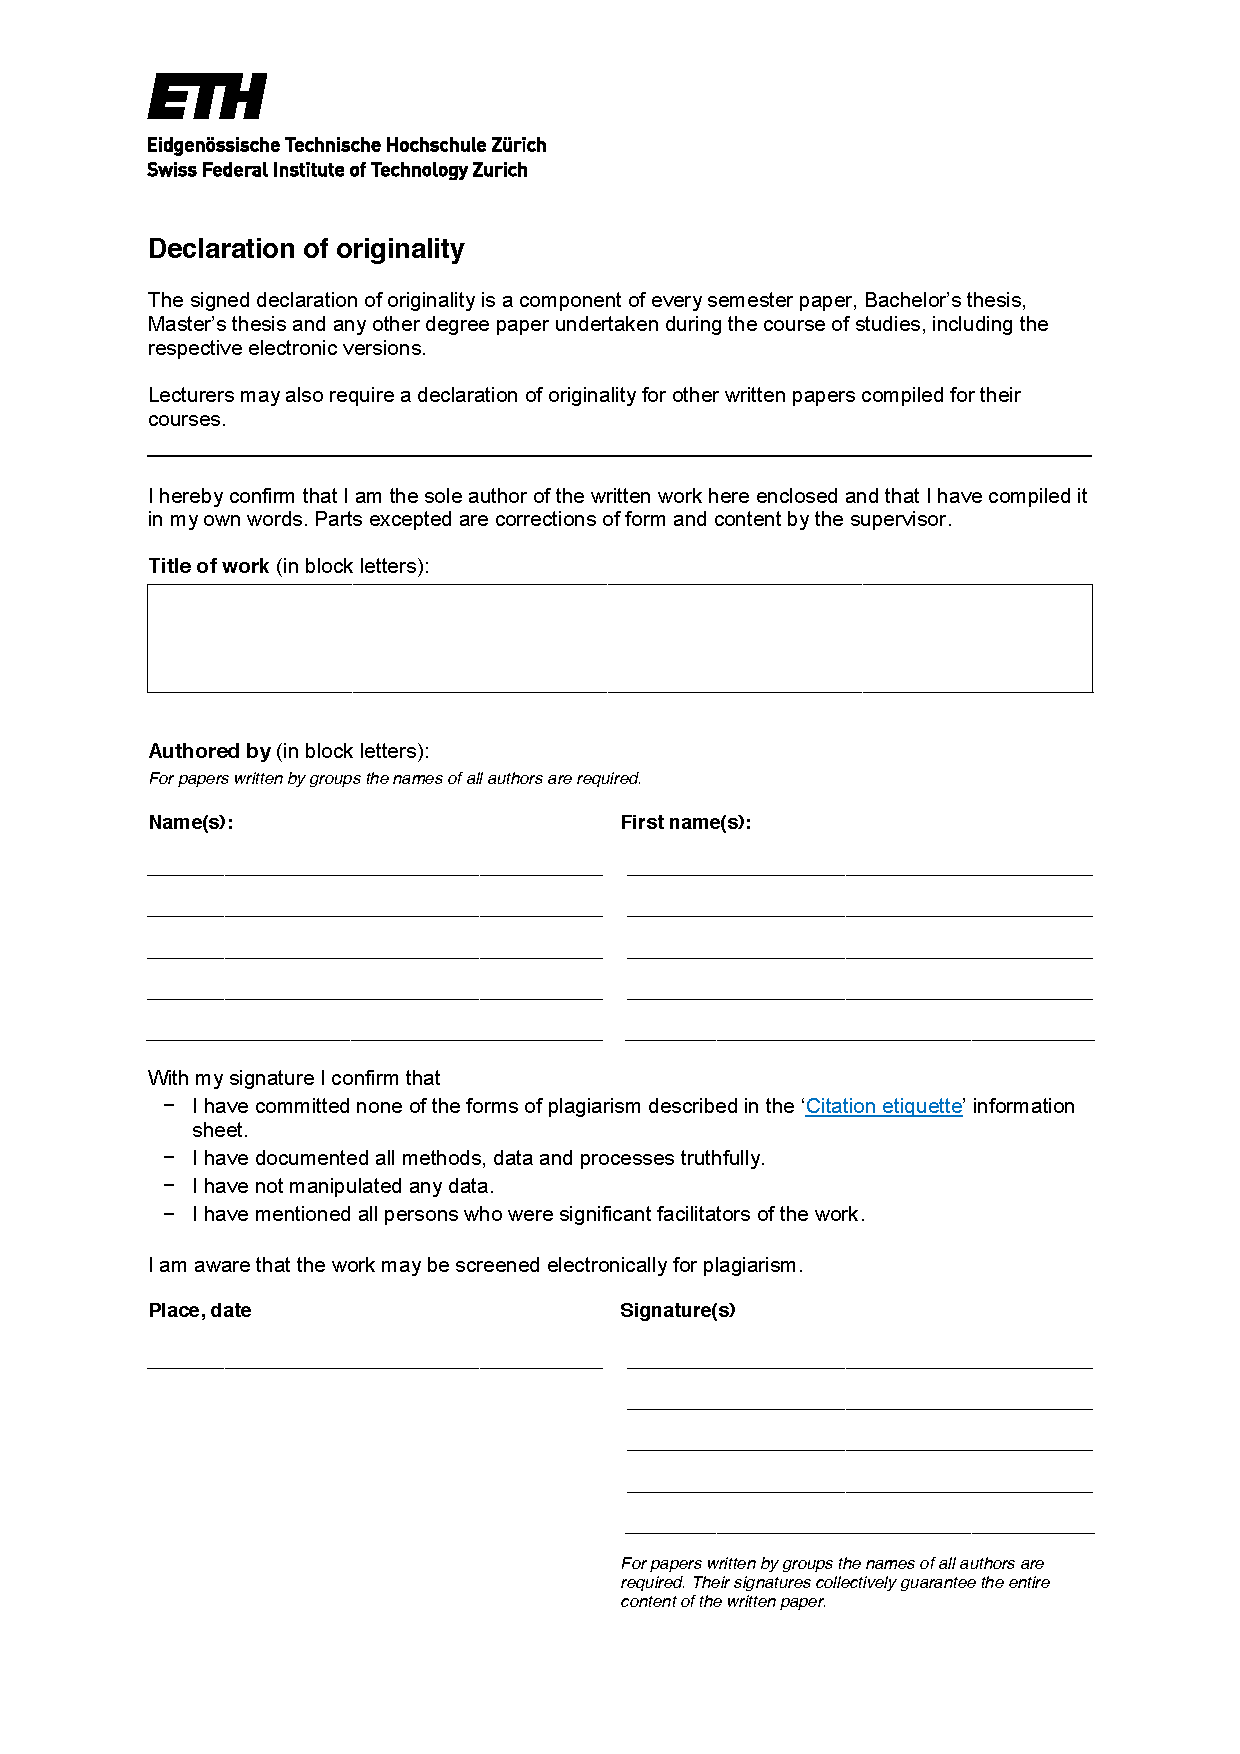
\includepdf[pages={-}]{declaration-originality.pdf}

\end{document}
